\documentclass[a4paper,12pt]{article}

%Preambulo, importar pacotes (de lingua)
\usepackage[brazil]{babel}
\usepackage[T1]{fontenc}
\usepackage[utf8]{inputenc}
\usepackage{lmodern}
\usepackage{graphicx}
\usepackage{booktabs}
\usepackage{siunitx}
\usepackage{caption}
\usepackage{textcomp}
\usepackage{subcaption}
\usepackage{listings}
\usepackage{amssymb}
\usepackage{subfig}
\usepackage{setspace}
\usepackage{longtable}
\usepackage{helvet}
\renewcommand{\familydefault}{\sfdefault}

\begin{document}

\begin{quote}
\centering
UNIVERSIDADE FEDERAL DE VIÇOSA\\
CENTRO DE CIÊNCIAS EXATAS E TECNOLÓGICAS\\
DEPARTAMENTO DE INFORMÁTICA\\

\large 
\

\

RESEARCH PROJECT

\

\
%towards an offline GPS trajectory preproscessing framework for trajectories storage 
\centering 
A TRAJECTORY DATA PREPROCESSING FRAMEWORK FOR TRAJECTORIES STORAGE AND ANALYSIS\\

\

\

\

\
\normalsize
\begin{flushright}
\textbf{Douglas Alves Peixoto}\\ 
MSc Student in Computer Science
\end{flushright}

\

\

\
Jugurta Lisboa Filho \\
(Advisor)
\

\

\

\
Fabio Ribeiro Cerqueira \\
(Co-Advisor)
\

\

\

\

\
VIÇOSA - MINAS GERAIS\\
NOVEMBER - 2014
\end{quote}

\newpage    % quebra de pagina

\onehalfspacing       % 1.5 line spacing
\tableofcontents      % Gera o sumario

\newpage    % quebra de pagina

\section{INTRODUCTION}\label{sec:intro}
The study of GPS trajectory data has become an important field of study in computer science due to the increasing volume of spatio-temporal data obtained from mobiles and GPS devices, which provide options for users to store their mobility log. This the massive amount of data to be analyzed has lead researchers to develop computational tools and data mining techniques combined with machine learning algorithms to enable a better management and understanding of mobile objects \cite{gudmundsson2012}.

The importance of the data mining studies for the modern society is to help individuals and companies to extract useful information from big data sets \cite{han2011}\cite{rajaraman2012}, which is manually impracticable; hence, these techniques can be likewise applied to analyze spatial data in a large scale. One example of an application of trajectory data analysis is to understand human behavior and movement patterns in urban areas.

Although many efforts have been done to analyze trajectories, not much have been done to pre-process these huge amount of data \cite{alvares2009}\cite{idrissov2012}. Data preprocessing aims to prepare the data beforehand, mainly by means of statistical and data mining techniques, for its further analysis; such preprocessing techniques may include detection and removal of noise, data reduction and data integration. Raw spatial data are subjected to inconsistencies and noise due to GPS imprecision or device failure, poor data modeling, human mistake, and database problems among others. Even though there are many sources of trajectory data available, e.g. \cite{nokia2012}\cite{yuan2010}\cite{zheng2010}, these data are generally sparse and usually do not combine due to schema mismatch. Therefore, data preprocessing plays an important role into data analysis and storage, once it aims to provide a trustful, integrated, clean and quality data to be stored and accurately analyzed.

In the scope of this project we are going to carry out an study of data preprocessing techniques, in special data integration, data cleaning and data reduction, and apply it on real trajectory datasets. The goal is to propose a trustful framework for trajectory data preprocessing aiming its further storage without loss of information, that is, after the preprocessing we must make sure that the semantic of the data is kept. Figure~\ref{fig:fig1} illustrates the steps of the proposed framework, which will be further described in this work.

% Figure 1 - overview
\begin{figure}[htb]
\centering
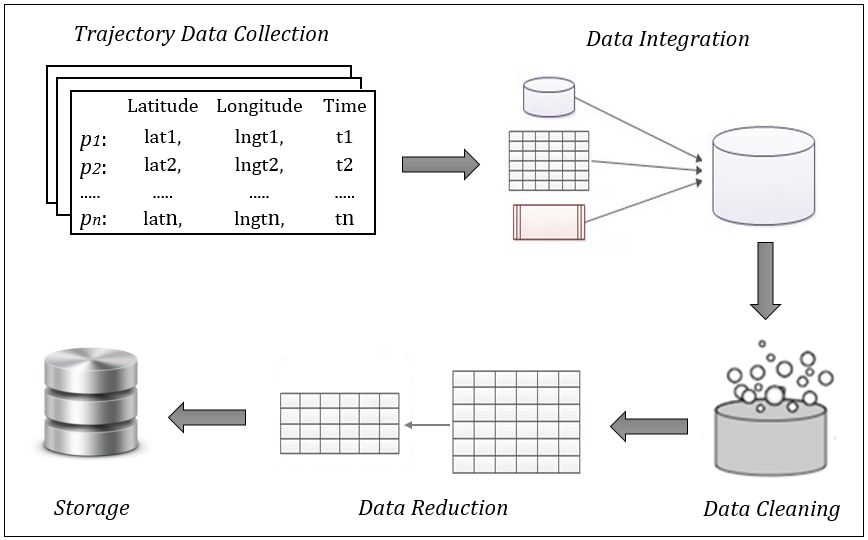
\includegraphics[width=1\textwidth]{overview}
\caption{Framework steps overview.}
\label{fig:fig1}
\end{figure}

The remainder of this paper is organized as follows. In Section~\ref{sec:relatedwork} we discuss the related work. Section~\ref{sec:methodology} describes the methodology to build up our framework, addressing every step for trajectory data preprocessing proposed in this project, while Section~\ref{sec:validation} presents the steps to be followed for the experimental validation of the proposed framework. Finally, we conclude presenting the timeline and the planned budget for this research project in Sections \ref{sec:timeline} and \ref{sec:budget} respectively. 
 
\section{RELATED WORK}\label{sec:relatedwork}
Despite the considerable amount of work proposed to analyze GPS trajectories, e.g. \cite{chen2011}\cite{gudmundsson2012}\cite{yuan2010}\cite{zheng2008}\cite{zheng2009}, and to store and share huge amount of spatial data, such as Spatial Data Warehouses (SDW) \cite{barclay2000}, Spatial Data Infrastructures (SDI) \cite{oxford2000}\cite{rajabifard1999} and Geographic DBMS (e.g. Oracle Spatial and PostGIS), to our best knowledge not many efforts have been done specifically to address the problem of preprocessing trajectory data, in particular focused on trajectories storage.

Alvares et al.~\cite{alvares2009}, for instance, present a framework for trajectory data preprocessing, their goal is to provide a framework for applications that aim the semantic analysis and mining of trajectory data in a high level of abstraction. In \cite{alvares2007} the authors proposed a model for enriching trajectories with geographic semantic information. According with with Alvares et al.~\cite{alvares2007}, devices for collection of trajectories of moving object do not aim to collect the geographic semantic information. Based on this statement, the authors introduce a framework for preprocessing trajectories aiming to add meaningful characteristics on them, based on the trajectory speed and places that the trajectory intersect. Although it is not in the scope of our preprocessing framework to neither add nor remove semantic information from trajectories, no doubt whatsoever the Alvares et al.~\cite{alvares2007}\cite{alvares2009} approaches can be used as an addition to our framework to enrich trajectories with semantic, before a trajectory data mining or analysis in a high level of abstraction. 

In another work Idrissov and Nascimento \cite{idrissov2012} present a framework for cleaning trajectories focused on trajectory data clustering. The framework is divided into three steps: stop detection, missing segment interpolation and inaccuracy removal. Although the framework demonstrates an improvement on trajectory data quality for clustering, it uses some approaches that may affect the semantic of the trajectory, such as the stop detection step, which aims to detect stops on the trajectory and remove them in order to improve the accuracy of clustering algorithms. However, some methods for trajectory data mining, such as Zheng et al. \cite{zheng2009} uses stops to detect points of interest in cities. Bearing it in mind, we propose a framework for preprocessing trajectories without semantic loss.

Additional work in the literature have been found to address on-line trajectory preprocessing and analysis \cite{fazzinga2014}\cite{lange2008}\cite{pumpichet2012}, which aim to deal with data on-the-fly, that is, while the collector devices, such as Radio-Frequency IDentification (RFID) \cite{fazzinga2014} and Stream Sensors \cite{pumpichet2012}, are still receiving the data. Our proposed framework is to deal with off-line preprocessing, once we are going to carry out our methodology on datasets from which the data have already been collected. Methodologies to deal with on-line data preprocessing and analysis differ from ours, for they aim to make predictions on data on-the-fly, so that they can detect anomalies and outliers on the data while it is being collected  by means of statistical inference.

A few other works have focused on trajectory outlier detection \cite{deAquino2013}\cite{fontes2013} \cite{gupta2014}\cite{lee2008}. However, these works aim on identify trajectories that deviates from a standard path or trajectory dataset pattern, not on preprocessing neither on identifying outliers in the trajectory itself.

To sum up, in this work we intent to study the WEKA toolkit, which is a free Java library for machine learning and data mining. This toolkit have been extended to deal with geographic data mining, including some preprocessing techniques \cite{bogorny2006weka}.

\section{METHODOLOGY}\label{sec:methodology}
As previously stated, the objective of this research is to provide a framework for preprocessing GPS trajectory data without loss of semantic. Provide clean, integrated, reduced and quality data for trajectories storage and analysis.

In this section we describe the methodology that shall be adopted to achieve the goals of this work. This section is divided into five parts: at first, we briefly introduce the datasets which will be used in this project; secondly, we propose a conceptual model and rules to integrate trajectories into a single schema; next, we describe the statistical and other techniques used upon the data to address the problem of trajectory data cleaning; subsequently, we introduce some data reduction techniques, explaining how they can be handled to simplify a trajectory, reducing its size and still keeping its semantic; finally, we describe the methodology that will be used to validate our approach.

%The theoretical background for our methodology was extracted mainly from the following books: Data mining theory and methods for data preprocessing were extracted mainly from Han et al.~\cite{han2011}. Statistical methods and theory extracted mainly from Wackerly et al.~\cite{wackerly2007} and Wong and Lee~\cite{wong2005}. Linear Algebra fundamentals extracted mainly from Anton~\cite{anton2010} and Lay~\cite{lay2003}.

\subsection{Data Cleaning: Datasets}\label{sec:datasets}
In this project we are going to work with real trajectory datasets instead synthetic data to carry out our experiments, for they better represent the reality (e.g. real-world traffic flows and traffic jams) and are more prone to noise. Trajectories of moving objects can be in most of cases represented as an ordered set of vertexes $p_i = (x_i, y_i, t_i)$ inputs. In other words, a trajectory $\tau$ with $n$ coordinate points is given by $\tau = \{p_1, p_2, \dots, p_n\} = \{(x_1, y_1, t_1), (x_2, y_2, t_2), \dots,(x_n, y_n, t_n)\}$, where $(x_i, y_i)$ are the coordinates of the $i_t$$_h$ trajectory vertex $p_i$ (e.g. latitude and longitude), and $t_i$ is the coordinate time-stamp. The datasets which will be used in this work are presented as follows:
 
\subsubsection{GeoLife Dataset}\label{sec:geolife} 
In this section, we briefly introduce the Microsoft's GeoLife networking service, Zheng et al.~\cite{zheng2010}. The GeoLife dataset recorded a broad range of users' outdoor movements, including not only life routines like go home and go to work but also some entertainments and sports activities. It is a very popular trajectory data source due to its variety and flexibility of data.

The GeoLife dataset contains GPS trajectories collected by Microsoft Research Asia among 182 individuals distributed in over 30 cities of China and in some cities located in the USA and Europe in a collaborative manner \cite{geolifeuserguide}. Information about this dataset is shown in Table 1. The data was collected in a period over five years (April 2007 to August 2012) and were recorded by different devices such as GPS loggers and GPS-phones. The trajectories in this dataset are composed by a sequence of raw GPS coordinates with latitude, longitude and time-stamp. The majority of these trajectories were recorded in a dense time and distance interval, i.e. every $1\sim5$ seconds or every $5\sim10$ meters per coordinate.
	
\begin{table}[htbp]
\centering
\label{tab:geolife}
\begin{tabular}{cc}
\toprule
\multicolumn{2}{c}{GeoLife Dataset}\\
\midrule
Number of Users	& 182\\
Number of Trajectories & 18.670\\
Number of Coordinates & 24.876.978\\
Total Distance & 1.292.951 km\\
Total Duration & 50.176 hours\\
Effective Days & 11.129\\
\bottomrule
\end{tabular}
\caption{GeoLife Dataset Info.}
\end{table}
	
\subsubsection{T-Drive Dataset}\label{sec:tdrive}
The T-Drive dataset contains GPS trajectories of of over 33,000 taxis during a 3 months period of 2008 within the city of Beijing. The total number of points in this dataset is about 15 million and the total distance of the trajectories reaches to 9 million kilometers. The average sampling interval is about 177 seconds with a distance of about 623 meters. This dataset have been efficiently used to mine fast routes to a given destination based on the experience of taxi drivers \cite{yuan2011}\cite{yuan2010}.

\subsection{Data Integration}\label{sec:integration}
From collecting trajectory data from different sources, problems may occur when merging these data into a single dataset, due to modeling divergences on each source schema. The analysis of the data should be carried out in a single coherent dataset for the sake of efficiency and simplicity, but each dataset may have been modeled into a different schema, and their variables and tuples shall probably not match perfectly into a single schema, even though the data sources are related to a same domain. The same problem aforementioned occurs with spatial data.

In the second part of this project we aim to provide a methodology and a schema to integrate GPS trajectories from different sources, by selecting and keeping into the schema only those fields that are worth to be stored and important for the analysis of the data, such as latitude, longitude and timestamp. The conceptual data schema for trajectory integration proposed in our framework is shown in Figure~\ref{fig:fig2}. Spaccapietra et al. \cite{spaccapietra2008} present two models for representing trajectories from a conceptual point of view. Although the models also take the semantic representation of trajectories into account, both models focus on their geometric representation, and were mainly designed for Geographic DBMS. In our framework we sole intent to provide a model for integrate trajectories, by keeping those fields which are essential for a trajectory representation and analysis, and are mostly available from all trajectory datasets. The conceptual model of Figure~\ref{fig:fig2} was build using the UML GeoProfile \cite{sampaio2010}, which was designed for modeling of geographic databases using UML diagrams.

% Figure 2 - integration model
\begin{figure}[htb]
\centering
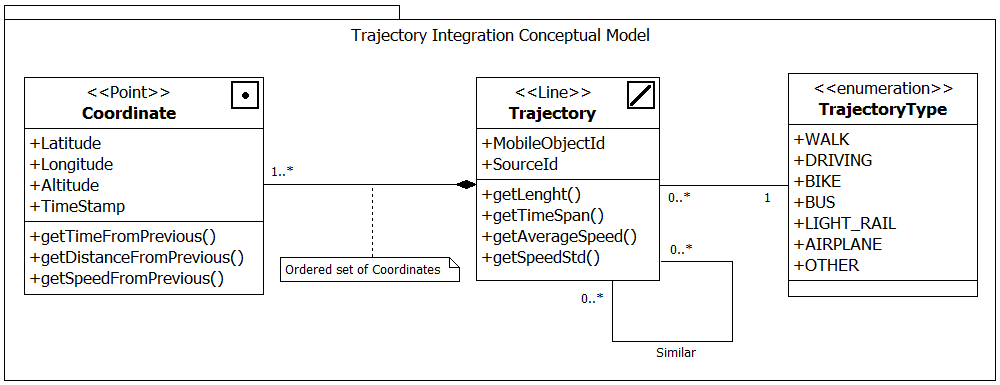
\includegraphics[width=1\textwidth]{integration_model}
\caption{Trajectory Integration Conceptual Model.}
\label{fig:fig2}
\end{figure}

During the process of integration some redundancy may be detected (i.e. similar trajectories); correlation analysis should be carried out to detect those redundancies \cite{han2011}. The problem of detecting similar trajectories play an important role in trajectory storage and analysis; for this reason, a data correlation analysis will be taken into account during the data integration process, which is described later.

The steps to be followed in our integration methodology are briefly described as follows:

\begin{enumerate}
	\item From all datasets, extract the attributes pursuant to the conceptual model of Figure~\ref{fig:fig2}.
	
	\item \textit{Latitude} and \textit{Longitude} attributes will be kept in decimal degrees, or converted if they are not yet.
	
	\item The \textit{Altitude} attribute, when applied, will be kept, or converted, into meters, or will receive a NULL value if it is missing or not valid.
	
	\item \textit{TimeStamp} attribute of each coordinate will be kept, or converted, into the number of days (with fractional part) that have passed since 01/01/1900.
	
	\item We will use GMT (Greenwich Mean Time) in the TimeStamp attribute of all coordinates, as in the GeoLife dataset, to avoid potential confusion of time zone.
	
	\item  All trajectories must be associated with a type of trajectory, which are represented in the enumeration of Figure~\ref{fig:fig2}. This will be useful for further preprocessing steps and future data analysis. If the type is unknown, or different from those represented in the model, one must set it as ``OTHER''. More trajectory types can be added to the \textit{TrajectoryType} enumeration according with the data sources one is working with. 
	
	\item  All trajectory objects in the model contain three attributes named~\textit{MobileObjectId} and \textit{SourceId}, which refer to the origin of the trajectory. For instance, in this project all the trajectories from the GeoLife dataset will have the \textit{SourceId} attribute tagged as ``GEOLIFE'', the attribute \textit{MobileObjectId} is the mobile object identifier whose the trajectory was generated from (can be a person, a vehicle, a device, or something else). The same will be done for all other datasets that will compose the integrated schema.
	
	\item The methods \textit{getLength()}, \textit{getTimeSpan()}, \textit{getAverageSpeed()} and \textit{getSpeedStd()} belonging to the class \textit{Trajectory}, return respectively the length of the trajectory in meters; its time span, that is, the time-stamp of its last coordinate minus the time-stamp of its first coordinate; its average speed and its standard deviation speed.
	
	\item The methods belonging to the class \textit{Coordinate}, namely, \textit{getTimeFromPrevious(), getDistanceFromPrevious()} and \textit{getSpeedFromPrevious()} from Figure~\ref{fig:fig2}, return, respectively, for a coordinate $p_i$, the time taken, the distance, and the speed from the coordinate $p_{i-1}$, and are for use in the cleaning process, which will be described later.
\end{enumerate}

\subsubsection{Check Trajectories Similarity}\label{sec:similarity}
During the process of integration, some redundancy among trajectories may be detected; similarity analysis should then be carried out to detect those redundancies during the data integration process in order to group similar trajectories. The relationship \textit{Similar} in Figure~\ref{fig:fig2} was created to address this issue.

Redundancy sometimes can be important for trajectory analysis; for instance, one may be interested in planning a road network capacity, planning municipal transportation or detect usual road paths in a city to avoid traffic jam \cite{deAquino2013}. In this sort of analysis, redundant trajectories are important, and should not be removed from the dataset, rather they should be grouped according with some similarity criteria chosen by the user of the framework. On the other hand, depending on the problem one is modeling, and the purpose of the pre-processing, this approach can be used to provide a set of disjoint trajectories instead, by removing redundant trajectories.

The definition of similarity depends on the sort of problem one is interested in; for instance, one may be interested in grouping, or removing, trajectories that are geographically identical, as shown in Figure~\ref{fig:fig3} (a); or group them by location, that is, all trajectories within a given spatial range are similar; one may also be interested in grouping trajectories which move along the same road or direction, for instance, all trajectories that cross the Wall Street in NY are similar, or trajectories that move towards Sydney in Australia are likewise similar. The end user is free to define the similarity criteria that better suits the problem. 

One common way to compare time-series objects (i.e. trajectories) is by means of Dynamic Time Warping (DTW) \cite{berndt94}, which can be used to evaluate the distance between two objects that have the same pattern but different speeds. Several other efforts have been done to evaluate similarity between trajectories based on curve similarity, e.g. \cite{buchin2009}\cite{liu2012}\cite{sankararaman2013}\cite{siirtola2008} \cite{tiakas2009}\cite{vanKreveld2007}\cite{vlachos2002ICDE}\cite{vlachos2002DEXA}. 

Although the aim of this framework at this point is to sole provide a methodology to integrate trajectory datasets, it is intended to make a comparative study among methods to detect similar trajectories based on curve similarity. When comparing similarity among curves, three situations may happen, and we must approach them differently, they are shown in Figure~\ref{fig:fig3}. As an example, lets take two trajectories, $\tau_a$ and $\tau_b$, defined as an ordered set of time-stamped coordinate points as follows:

\[
	\tau_a = \{p_{a1}, p_{a2}, p_{a3}, ..., p_{an}\},~~\tau_b = \{p_{b1}, p_{b2}, p_{b3}, ..., p_{bn}\}
\]

% Figure 3 - similarity
\begin{figure}[htbp]
	\centering
	\begin{subfigure}{0.32\textwidth}
		 \centering
		 \label{fig:fig3a}
		 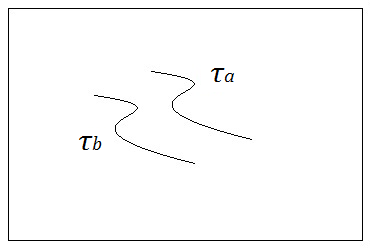
\includegraphics[scale=0.6]{similar_a}
		 \caption{}
	\end{subfigure}
	\hfill 
	\begin{subfigure}{0.32\textwidth}
		 \centering
		 \label{fig:fig3b}
		 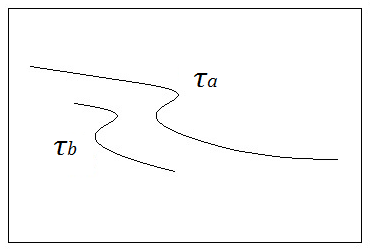
\includegraphics[scale=0.6]{similar_b}
		 \caption{}
	\end{subfigure}
	\hfill 
	\begin{subfigure}{0.32\textwidth}
		 \centering
		 \label{fig:fig3c}
		 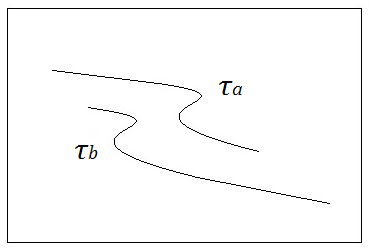
\includegraphics[scale=0.6]{similar_c}
		 \caption{}
	\end{subfigure}	
	\caption{Curve Similarity.}
	\label{fig:fig3}
\end{figure}

The first scenario, shown in (a), occurs when both trajectories, $\tau_a$ and $\tau_b$, are very similar (according with a similarity threshold $\varepsilon$), or identical, that is, $\tau_a = \tau_b$. The second scenario, shown in (b), occurs when one of the trajectories is longer, in one side or both sides, than the other trajectory, that is, $\tau_a \subset \tau_b$ or $\tau_b \subset \tau_a$. The last scenario, shown in (c), occurs when both trajectories are longer than the other one but in different directions. For each pair of similar trajectories, we label its type and set the degree of similarity pursuant to the scenario. 

\subsection{Data Cleaning}\label{sec:cleaning}
Data in real world tend to be noisy, inconsistent and/or incomplete due to a variety of issues that may happen during the process of collection, modeling and storage of the data, and also due to human mistakes and collection devices error. Data cleaning techniques aim to work on this problems, by filling in missing values, identifying and correcting inconsistencies, and smoothing noise \cite{han2011}. The main objective of data cleaning is to increase the accuracy of a further analyses of the data; cleaned datasets can also improve data matching. There are a considerable amount of data mining techniques do deal with noisy in a broad range of fields; Chapman \cite{chapman2005cleaning}, for instance, present a survey on techniques for cleaning databases of insect species based on their geographic occurrence; in another work, the author present techniques for data quality in spatial data \cite{chapman2005quality}, arguing that quality is merely a factor of fitness for use or potential use, and it is relative to the domain and purpose one is interested in. 

The goal of this cleaning process is to provide more trustful, accurate and quality trajectory data to be analyzed and stored without loss on its semantic. Missing and incorrect attribute values contribute for inaccurate trajectory data analysis and a poor data storage, as well as do noisy coordinates. To address the problem of trajectory data cleaning, in our framework we propose an approach for cleaning trajectories in a four step process, namely: (1)~remove duplicate coordinates, (2)~remove inconsistent values, (3)~predict missing values, and (4)~identify and ignore noisy coordinates. 

\subsubsection{Preliminaries}\label{sec:preliminaries}
Before we can start, let us introduce some basic terminology. Let $I$ be our integrated set of trajectories as described in Section~\ref{sec:integration}, and lets suppose our set $I$ contains $k$ trajectories, that is $|I| = k$. For the sake of brevity, we are going to present our cleaning process for a single trajectory $\tau$ with $n\in\mathbb{N^*}$ coordinate points. However, all the steps described here will be performed for all $\tau_i \in I$, where $i = \{1, 2, \dots, k\}$.

Therefore, given a trajectory $\tau \in I$ with $n\in\mathbb{N^*}$ coordinate points, let $p_i = (x, y, t)$ be the $i_{th}$ coordinate of $\tau$, where $x$ and $y$ denotes the geographic object's position at time $t$. We define $t(i)$, $d(i)$ and $s(i)$ respectively as the time taken in seconds~(s), the distance in meters~(m) and the speed in meters per second~(m/s) from a coordinate point $p_{i-1}$ to $p_i$ of $\tau$ as follows:

	\[ t(i) = \left\{ \begin{array}{ll}
			0, & \mbox{if i = 1}\\
		    p_i.t - p_{i-1}.t, & \mbox{if i > 1}
	\end{array} \right. \]

	\[ d(i) = \left\{ \begin{array}{ll}
			0, & \mbox{if i = 1}\\
		    dist(p_{i-1}, p_i), & \mbox{if i > 1}
	\end{array} \right. \]
	
	\[ s(i) = \left\{ \begin{array}{ll}
			0, & \mbox{if i = 1}\\
		    d(i) / t(i), & \mbox{if i > 1}
	\end{array} \right. \]
	
Because we are dealing with spherical geometry, the $dist(p_{i-1}, p_i)$ function we use here, which returns the distance from $p_{i-1}$ to $p_i$ on a sphere (Earth), is the $Haversine Distance$, which calculates a great-circle distance between two points on a sphere from their  latitudes and longitudes. For any two points $p_i$ and $p_j$ on a sphere the $Haversine Distance$ is given by:

	\[
		{dist(p_i, p_j) = 2r sin^{-1}(\sqrt{sin^2(\frac{x_i - x_j}{2}) + cos(x_i)cos(x_j)sin^2(\frac{y_i - y_j}{2})}})
	\]

where $r$ is the $Earth$ radius, $x$ and $y$ are respectively the latitudes and longitudes of the points $p_i$ and $p_j$. 

Finally, for each trajectory $\tau \in I$ with $n$ coordinate points, we define three sets, namely $T, D, S \subset \mathbb{R^+}$, one for each of the trajectory functions previously described, where $T = \{t_1, t_2, \dots, t_n\}$, $D = \{d_1, d_2, \dots, d_n\}$ and $S = \{s_1, s_2, \dots, s_n\}$, such that for each $i \in \{1, 2, \dots, n\}$ we have $t_i = t(i)$, $d_i = d(i)$ and $s_i = s(i)$.

\subsubsection{Data Transformation}\label{sec:transformation}
In the last step of our cleaning process, we are going to use a speed-based statistical model; for this purpose, we perform a transformation on the speed set $S$ to an appropriate form for cleaning. We will conduct a Min-Max linear transformation on the original set $S$, that is, $f_{mm} : S \rightarrow S'$, which aim to map each value of speed $s_i \in S$ to a new value $s'_i \in S'$ in a range [$newMin_S, newMax_S$] $\subset\mathbb{R^+}$, by computing $\forall s_i \in S$: 

\[ f_{mm}(s_i) = s'_i = \frac{s_i - min_S}{max_S - min_S}(newMax_S - newMin_S) + newMin_S \]

We chose the Min-Max normalization for it preserves the relationship among the original values \cite{han2011}. This relationship is important for our cleaning process, in order to keep the semantic of the trajectory. This transformation will neither affect nor persist to the dataset $I$, once the new feature set $S'$ will be used only during the cleaning process, moreover $S \cup S' \nsubseteq I$. 

\subsubsection{Data Cleaning Steps}\label{sec:cleaningsteps}
Following we briefly present the four steps proposed for our cleaning framework.

\paragraph{STEP 1: Removing Duplicate Coordinates.}
Here we must remove duplicate occurrences of coordinates in a same trajectory $\tau$. For instance, we must check if there are more than one coordinate with the same values for the attributes \textit{Latitude}, \textit{Longitude} and \textit{TimeStamp} in a same trajectory; if so, the duplicates must be removed. Coordinates of a trajectory with only \textit{Latitude} and \textit{Longitude} duplicated, but different \textit{TimeStamp} must not be removed, since a trajectory can cross the same point more than once at different times, and a moving object can stay still in a same position for a long time.

\paragraph{STEP 2: Removing Inconsistent Values.}
Remove inconsistent values that make no sense for the attributes value range. For instance, negative \textit{TimeStamp}; \textit{Latitude} out of range from -90 to 90 degrees; \textit{Longitude} out of range from -180 to 180 degrees; \textit{TimeStamp} of a coordinate $p_i \in \tau$ bigger than the \textit{TimeStamp} of a coordinate $p_{i+1} \in \tau$, that is, $p_{i+1}.t < p_i.t$; etc. All these inconsistent values must be removed and the missing values filled with an acceptable one. Step~3 will deal with missing values.

\paragraph{STEP 3: Predicting Missing Values.}
Missing and NULL values does not always imply that there is error in the data. But for the case of trajectories, we assume that all coordinate $p_i \in \tau$ must have at least the attributes \textit{Latitude}, \textit{Longitude} and \textit{TimeStamp}. The lack of any of these attributes would make no sense for a trajectory schema. \textit{Altitude} can be omitted if it has not been collected. If between two coordinates $p_i$ and $p_j$ of $\tau$ there are $n$ coordinates $\{p_{i+1}, \dots, p_{j-1}\}$ lacking their values for \textit{Latitude}, \textit{Longitude} and/or \textit{TimeStamp}, we predict the missing values by making a local smoothing, by means of interpolation methods. The simplest example of such a problem is to find a linear polynomial whose graph passes through two known distinct points $p_i$ and $p_j$, where we know beforehand that the missing values are between $p_i$ and $p_j$, and fit the missing values according with the linear function. One example to predict missing values by means of a linear function using local mean is shown below.

\begin{center}
\lstset{escapeinside={\%}{\%},basicstyle=\footnotesize,tabsize=5}
\begin{lstlisting}
		FOR k = i+1 to j-1 DO {
			%$ v(p_k) = v(p_{k-1}) + increment $%
		}
\end{lstlisting}
\end{center}

where $v(p_k)$ is the value of the attribute (i.e. \textit{Latitude}, \textit{Longitude}, \textit{TimeStamp} or \textit{Altitude} (if applied)) of the coordinate $p_k \in \tau$, and 

\[
	increment = \frac{mean}{n} = \frac{v(i)+v(j)}{2*n}
\]

One example of linear interpolation for $(x, y)$ attributes of a trajectory is shown in Figure~\ref{fig:fig4}, where the points $p_k$, $p_{k+1}$ and $p_{k+2}$ have been add between points $p_i$ and $p_j$ by estimation of their values for $x$~and~$y$. One drawback of this approach is that if the variables are very sparse, a linear interpolation function would not represent the missing data accurately, showing a high estimation error rate. In this case, it is customary to use a higher degree polynomial interpolation method, such as \textit{Lagrange-Polynomial} which can perform a smoother representation of a curve, or \textit{Ordinary Kriging} for attributes estimation, which take the spatial correlation among the points into account to minimize the estimation error rate. Other estimation methods that can be exploit here are \textit{Triangulation} and \textit{Inverse Distance} \cite{isaaks90}. We aim to use those methods in this work, and compare one to another about their efficiency and error rate to approximate missing values for each of the coordinate attributes aforementioned.
 	
% Figure 4 - trajectory interpolation
\begin{figure}[!ht]
\centering
\begin{subfigure}{0.49\textwidth}
 \centering
 \label{fig4a}
 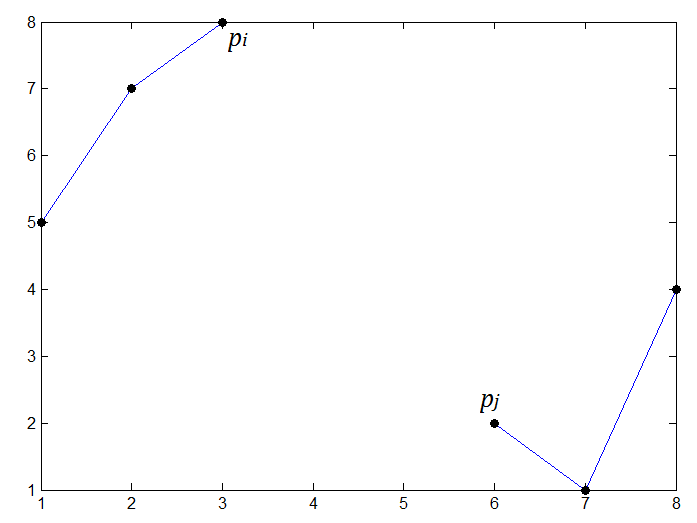
\includegraphics[scale=0.45]{interp1}
 \caption{Before Interpolation}
\end{subfigure}
\hfill 
\begin{subfigure}{0.49\textwidth}
 \centering
 \label{fig4b}
 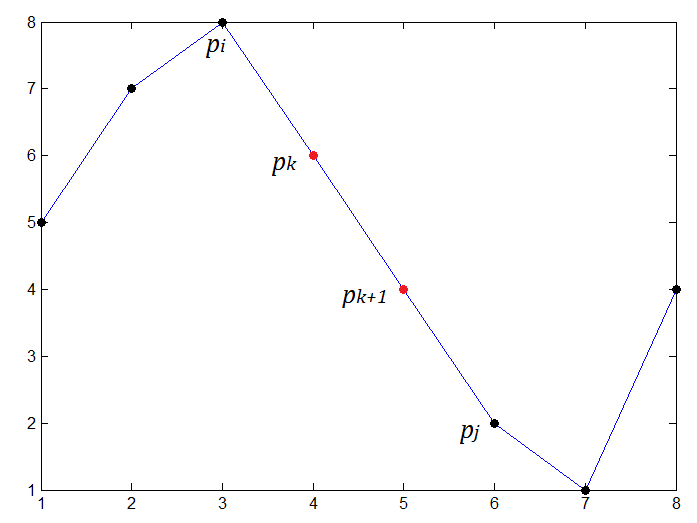
\includegraphics[scale=0.45]{interp2}
 \caption{After Interpolation}
\end{subfigure}
\caption{Example of Linear Interpolation}
\label{fig:fig4}
\end{figure}

\paragraph{STEP 4: Identifying and Ignoring Noisy Coordinates.}
In this final step of our cleaning process, we aim to remove noisy coordinates from trajectories. GPS trajectory data are quite susceptible to random noise for many reasons, such as human mistake, data transmission error and system or recording device error, among others. Figure~\ref{fig:fig5} (a) and (b) show two trajectories from the GeoLife dataset with some coordinates that deviates from the trajectory pattern; at one point a moving object suddenly took a very high speed, more than 200km/s, in period of less than 5 seconds, what is quite improbable. To remove this sort of noise, we are going to carry out an speed-based approach along the trajectories. 
	
% Figure 5 - trajectories
\begin{figure}[!h]
\centering
\begin{subfigure}{0.69\textwidth}
 \centering
 \label{fig:fig5a}
 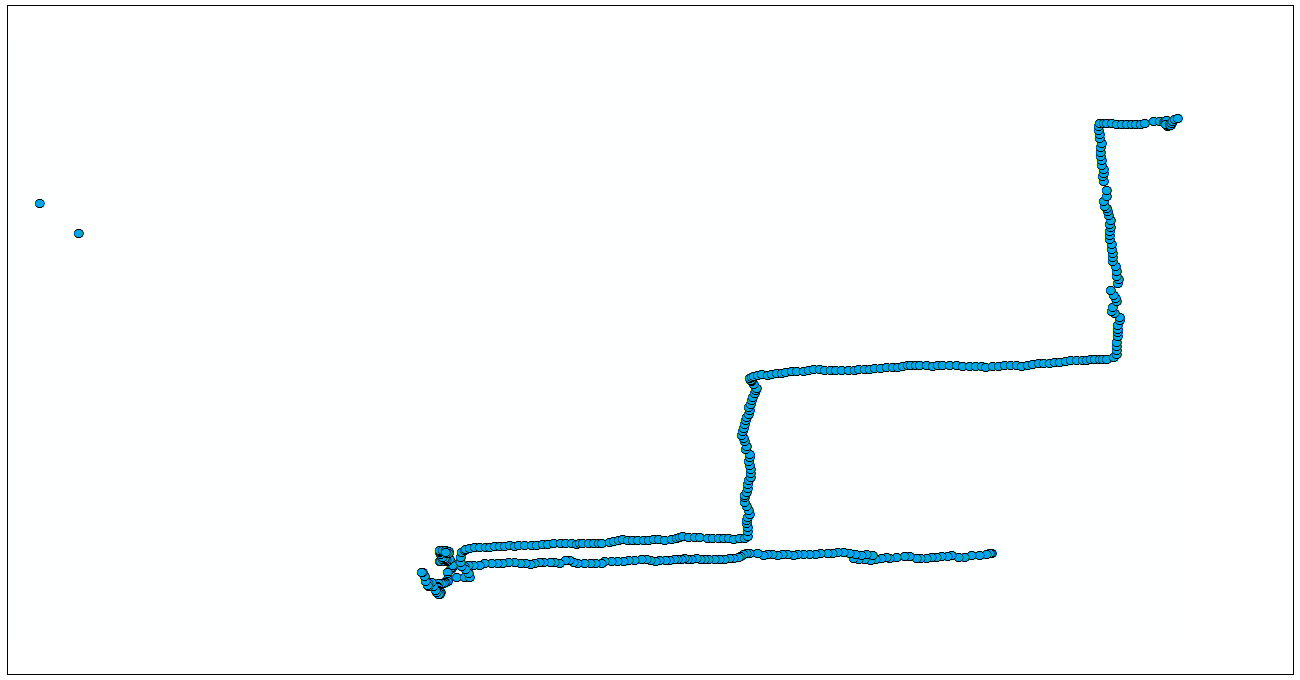
\includegraphics[scale=0.35]{traj1}
 \caption{}
\end{subfigure}
\hfill 
\begin{subfigure}{0.29\textwidth}
 \centering
 \label{fig:fig5b}
 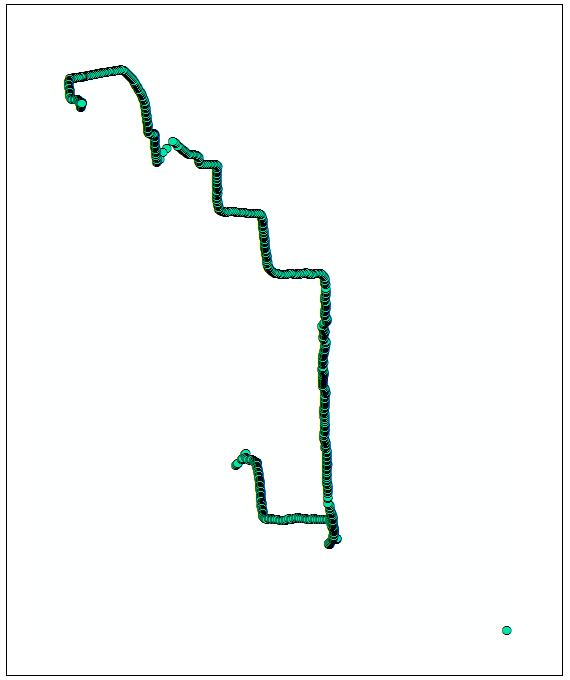
\includegraphics[scale=0.35]{traj2}
 \caption{}
\end{subfigure}
\caption{Noisy Coordinates}
\label{fig:fig5}
\end{figure}	
	
Firstly, we will calculate the speed set $S$ for a trajectory $\tau \in I$, as described in Section~\ref{sec:preliminaries}. Secondly, for the trajectory speed set $S$ we perform our transformation function $f_{mm} : S \rightarrow S'$ in order to get a normalized speed set $S'$, as described in Section~\ref{sec:transformation}. Finally, from $S'$ we check if in between any two coordinates the speed fluctuates to unacceptable values. To check for unacceptable values for speed, we are going to perform an statistical analysis of the distribution of the speed along the trajectory, that is, an statistical analysis of the elements of~$S'$. Coordinates such that its speed deviates too much from the speed distribution shall be removed.	

Figure~\ref{fig:fig6} shows the speed histogram along the trajectories of Figures~\ref{fig:fig5} (a) and (b) respectively. Figure~\ref{fig:fig7} shows the speed distribution (without normalization) for the trajectory of Figures~\ref{fig:fig5} (a) and (b) respectively. One may notice the anomalous fluctuation on the speed along the trajectories.
	
% Figure 6 - histogramas
\begin{figure}[!h]
%\centering
\begin{subfigure}{\textwidth}
 %\centering
 \label{fig:fig6a}
 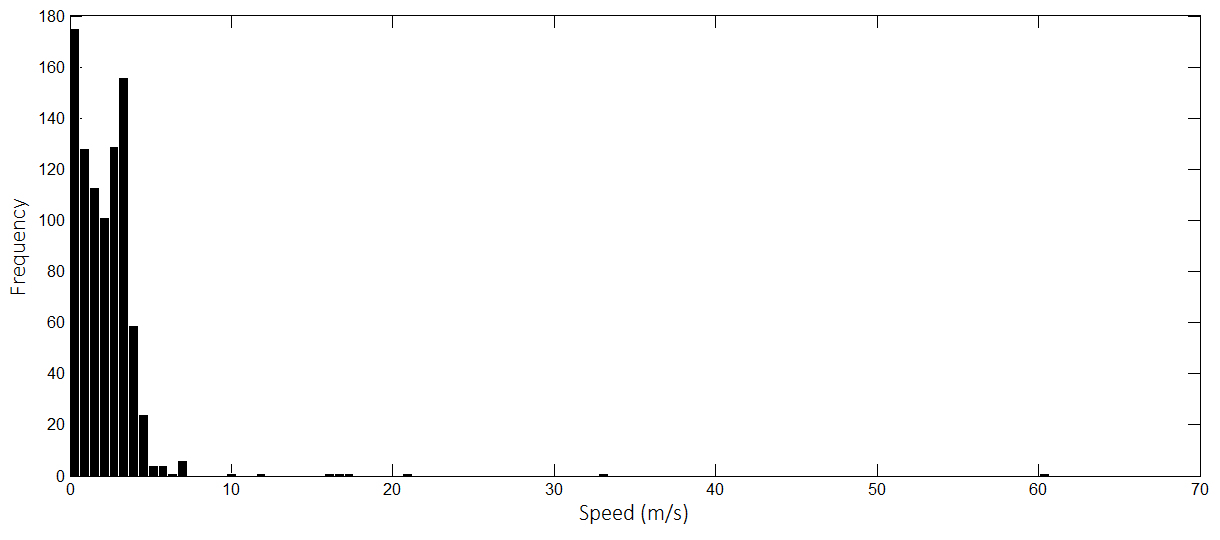
\includegraphics[scale=0.53]{hist1}
 \caption{}
\end{subfigure}
 
\begin{subfigure}{\textwidth}
 %\centering
 \label{fig:fig6b}
 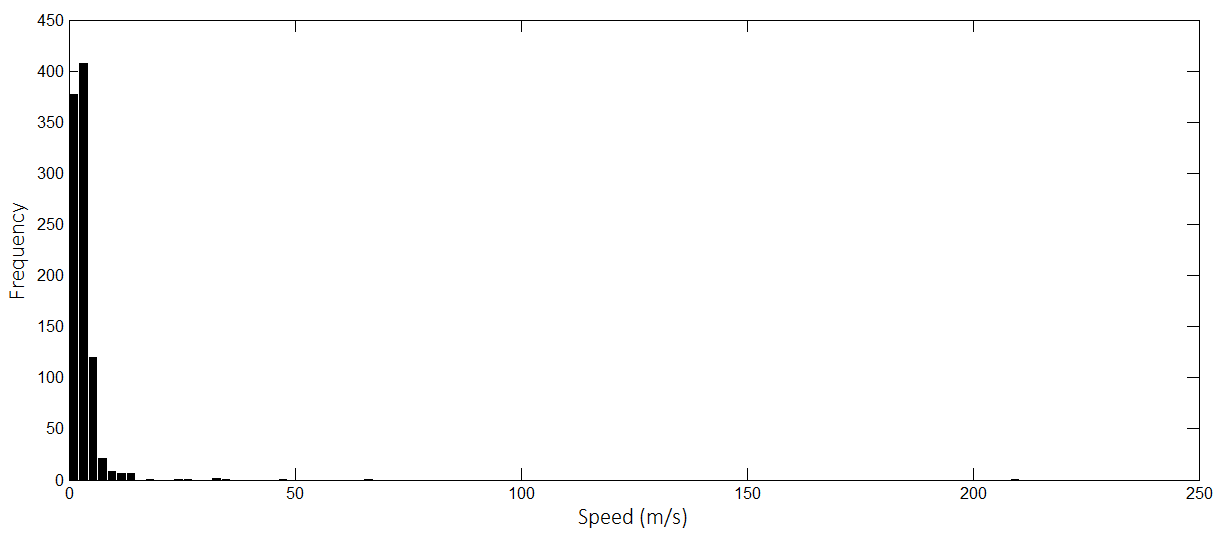
\includegraphics[scale=0.53]{hist2}
 \caption{}
\end{subfigure}
\caption{Trajectories Speed Histogram}
\label{fig:fig6}
\end{figure}

The goal at this step is to build a model $p(s)$ based on the normalized speed distribution $S' = \{s'_1, s'_2, \dots, s'_n\}$ of $\tau$ and find a threshold $\varepsilon$ such that $\forall p_i \in \tau$: 

\[ p_i = \left\{ \begin{array}{ll}
	noise, & \mbox{if $p(s'_i)  < \varepsilon$ }\\
	normal, & \mbox{if $p(s'_i) \geq \varepsilon$}
\end{array} \right. \]

For our anomaly detection approach, we can also apply another transformation on the speed distribution to make it close to a Gaussian distribution, and chose $\varepsilon$ based on its standard deviation $\sigma$, in other words $\varepsilon = c\sigma$, where $c \in \mathbb{N^*}$ is a constant. An additional approach to address this problem is to use a density-based algorithm for discovering both clusters and outliers on the speed distribution, such as the DBSCAN algorithm Ester et al.~\cite{ester96}, that is, cluster points by their speed using the point speed as distance function, so that points with similar speed will be put in a same cluster, whereas points with anomalous speed will be defined as outliers.

% Figure 7 - speed distribution
\begin{figure}[!h]
\centering
\begin{subfigure}{0.49\textwidth}
 \centering
 \label{fig7a}
 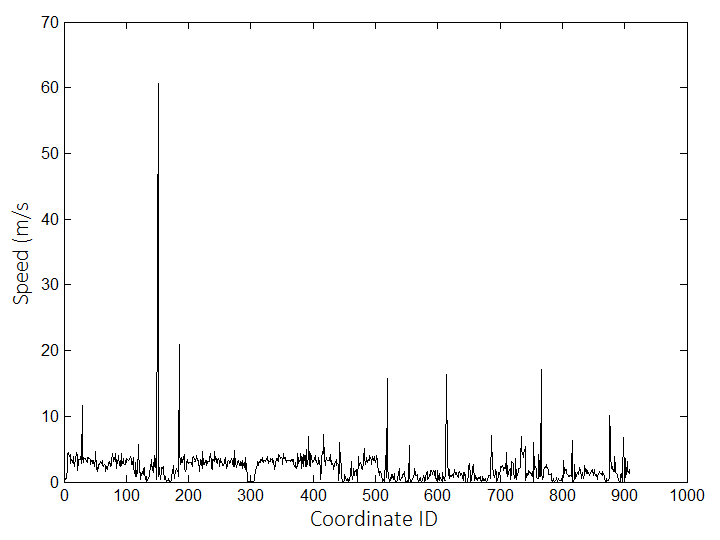
\includegraphics[scale=0.45]{speed1}
 \caption{}
\end{subfigure}
\hfill 
\begin{subfigure}{0.49\textwidth}
 \centering
 \label{fig7b}
 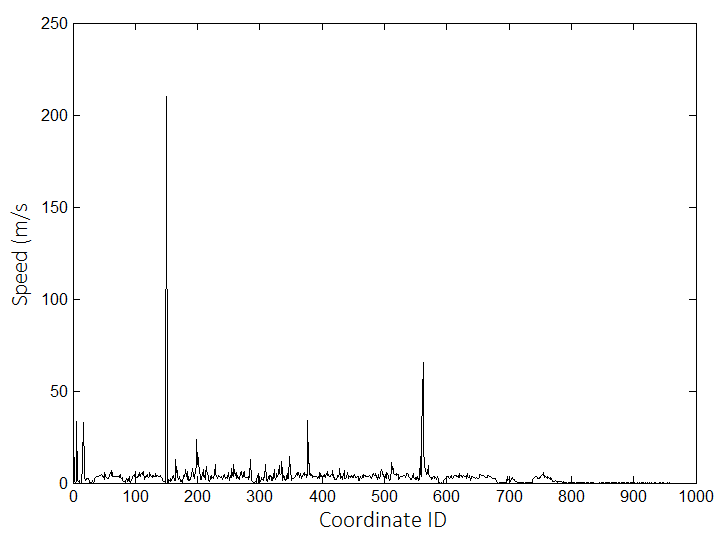
\includegraphics[scale=0.45]{speed2}
 \caption{}
\end{subfigure}
\caption{Trajectories Speed Distribution}
\label{fig:fig7}
\end{figure}

Finally, the step 3 of our cleaning process can be applied after the noise removal as well, to predict the right position for the noisy coordinates.

\subsection{DATA REDUCTION}\label{sec:reduction}
Trajectories may impose huge storage requirements. To address this problem, the final step of our framework is to carry out a trajectory data reduction focus on line-simplification approaches, such as the Douglas-Peuker heuristic~\cite{douglas73}. The goal of line-simplification approaches lies on approximate a trajectory by another one which is similar to the original, but has fewer points. This similarity is based on a predetermined accuracy bound $\varphi$, that is, the simplified trajectory deviates from the original one by less than a given accuracy bound $\varphi$. The value of $\varphi$ is also known in the literature as \textit{Haussdorff} distance, which measures how far two subsets in a two-dimensional space are from each other. Another well known algorithm for line-simplification that can be exploit in this project is the min-\# algorithm of Chen and Daescu \cite{chen98}. We aim with this approaches to reduce the trajectories storage consumption with a minimum or none information loss.

Figure~\ref{fig:fig8} shows a curve simplification using the Douglas-Peuker algorithm. This method has been shown to outperform other reduction methods, such as Wavelet Transforms and Log-Linear models~\cite{cao2006}. Besides, the integration process of our framework, presented in Section~\ref{sec:integration}, is also a data reduction approach, once it perform an attribute (or feature) subset selection method.

% Figure 8 - line simplification
\begin{figure}[!h]
	\centering
	\begin{subfigure}{0.49\textwidth}
		 \centering
		 \label{fig8a}
		 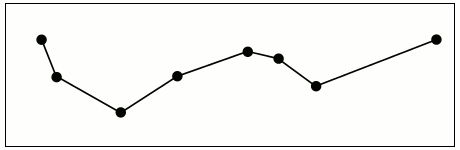
\includegraphics[scale=0.7]{reduce1}
		 \caption{Before Simplification}
	\end{subfigure}
	\hfill 
	\begin{subfigure}{0.49\textwidth}
		 \centering
		 \label{fig8b}
		 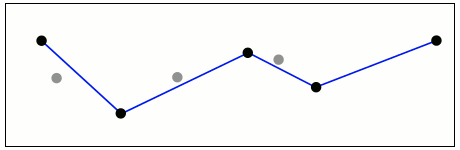
\includegraphics[scale=0.7]{reduce2}
		 \caption{After Simplification}
	\end{subfigure}
	\caption{Curve Simplification with Douglas-Peuker Heuristic}
	\label{fig:fig8}
\end{figure}

\section{EXPERIMENTAL VALIDATION}\label{sec:validation}
To validate our approach, we are going to carry out a comparative test between both our preprocessed trajectories and the original ones, by using them in a couple of recognized algorithms for trajectory analysis \cite{gudmundsson2012}\cite{zheng2008} \cite{zheng2009}, and compare their outcomes and performance for both set of trajectories. In addition, we shall compare our results with the methods for spatial preprocessing developed in the WEKA toolkit \cite{bogorny2006weka}. We expect that the outcomes of the algorithms show no expressive differences from one trajectory set to another, meaning that the semantic of the data is not affected by our preprocessing approach and there is no significant loss of information. On the other hand, we expect a significant drop in the storage requirements and a substantial increase in the performance of the algorithms aforementioned, once there will be less data to be stored and analyzed; hence, we expect a drop in the algorithms runtime.

\section{TIMELINE}\label{sec:timeline}

Table 2 shows the timeline for completion of major tasks for this research project, pursuant to the regulations from both the \textit{Pró-Reitoria de Pesquisa e Pós Graduação (PPG)} and the \textit{Departamento de Informática (DPI)}  to obtain the title of Master of Computer Science at the \textit{Universidade Federal de Viçosa (UFV)}.

\begin{table}[htbp]
\centering
\label{tab:timeline}
\begin{tabular}{l|c|c|c|c|c|c|c|}
\toprule
2015 & Jan & Fev & Mar & Apr & May & Jun & Jul \\
\midrule
Finish Literature Review & x & & & & & & \\
\midrule
Submit Short Paper & x & & & & & & \\
\midrule
Data Integration & x & x & & & & & \\
\midrule
Traj. Similarity Study & & & x & x & & & \\
\midrule
Traj. Data Cleaning & & & & & x & x & x \\
\midrule
Submit Short Paper & & & & & & & x \\
\midrule
\midrule
2015 & Aug & Sep & Oct & Nov & Dec & - & - \\
\midrule
Traj. Data Reduction & x & x & & & & & \\
\midrule
Experimental Validation & & & x & x & & & \\
\midrule
Dissertation Written & & & x & x & x & & \\
\midrule
Submit Paper Journal & & & & & x & & \\
\midrule
Dissertation Defense & & & & & x & & \\
\bottomrule
\end{tabular}
\caption{Research Project Timeline.}
\end{table}

\section{BUDGET}\label{sec:budget}

\begin{longtable}{lcc} %[htbp]
%\label{tab:budget}
%\begin{tabular}{lcc}
\hline
\textbf{Budget Specification} & \textbf{Amount R\$} & \textbf{Resources} \\
\hline
1 HUMAN RESOURCES & & \\
1.1 Allowance for execution of the research & 18.000 & CAPES\\
 (scholarship value x 12 months) & & \\
1.2 Advisor Committee (10\% of the salary  & & UFV\\
of the professors committee x 12 months) & - &  \\
\textbf{Subtotal} & \textbf{18.000} & \\
\hline
2 BIBLIOGRAPHIC MATERIAL & & \\
2.1 Books, technical journals, etc. & 1.000 & Own\\
\textbf{Subtotal} & \textbf{1.000} & \\
\hline
3 MATERIAL & & \\  
3.1 Reams of paper & 100 & Own \\ 
3.2 Ink cartridges for printer & - & - \\ 
3.3  CD and DVD  & - & - \\ 
\textbf{Subtotal} & \textbf{100} & \\
\hline
4 THIRD PARTY SERVICES & & \\  
4.1 Typing and formatting & - & - \\ 
4.2 Linguistic revision & - & - \\ 
4.3 Print/Bookbinding & 200 & Own \\ 
4.4 Post services & 100 & Own \\ 
\textbf{Subtotal} & \textbf{300} & \\
\hline
5 ACCOMMODATION & & \\
5.1 Field trip for data collection & - & - \\
\textbf{Subtotal} & \textbf{0} & \\
\hline
6 TECHNICAL RESERVE & & \\
6.1 10\% of the previous items & & Own\\ 
\textbf{Subtotal} & \textbf{1.940} & \\
\hline 
\textbf{Total} & \textbf{21.340} & \\
\hline
%\end{tabular}
\caption{Research Project Expected Budget.}
\end{longtable}

\bibliographystyle{acm}
\bibliography{bibliography}

\end{document}